\documentclass{standalone}
\usepackage{tikz}
\usetikzlibrary{arrows.meta, positioning}

\begin{document}
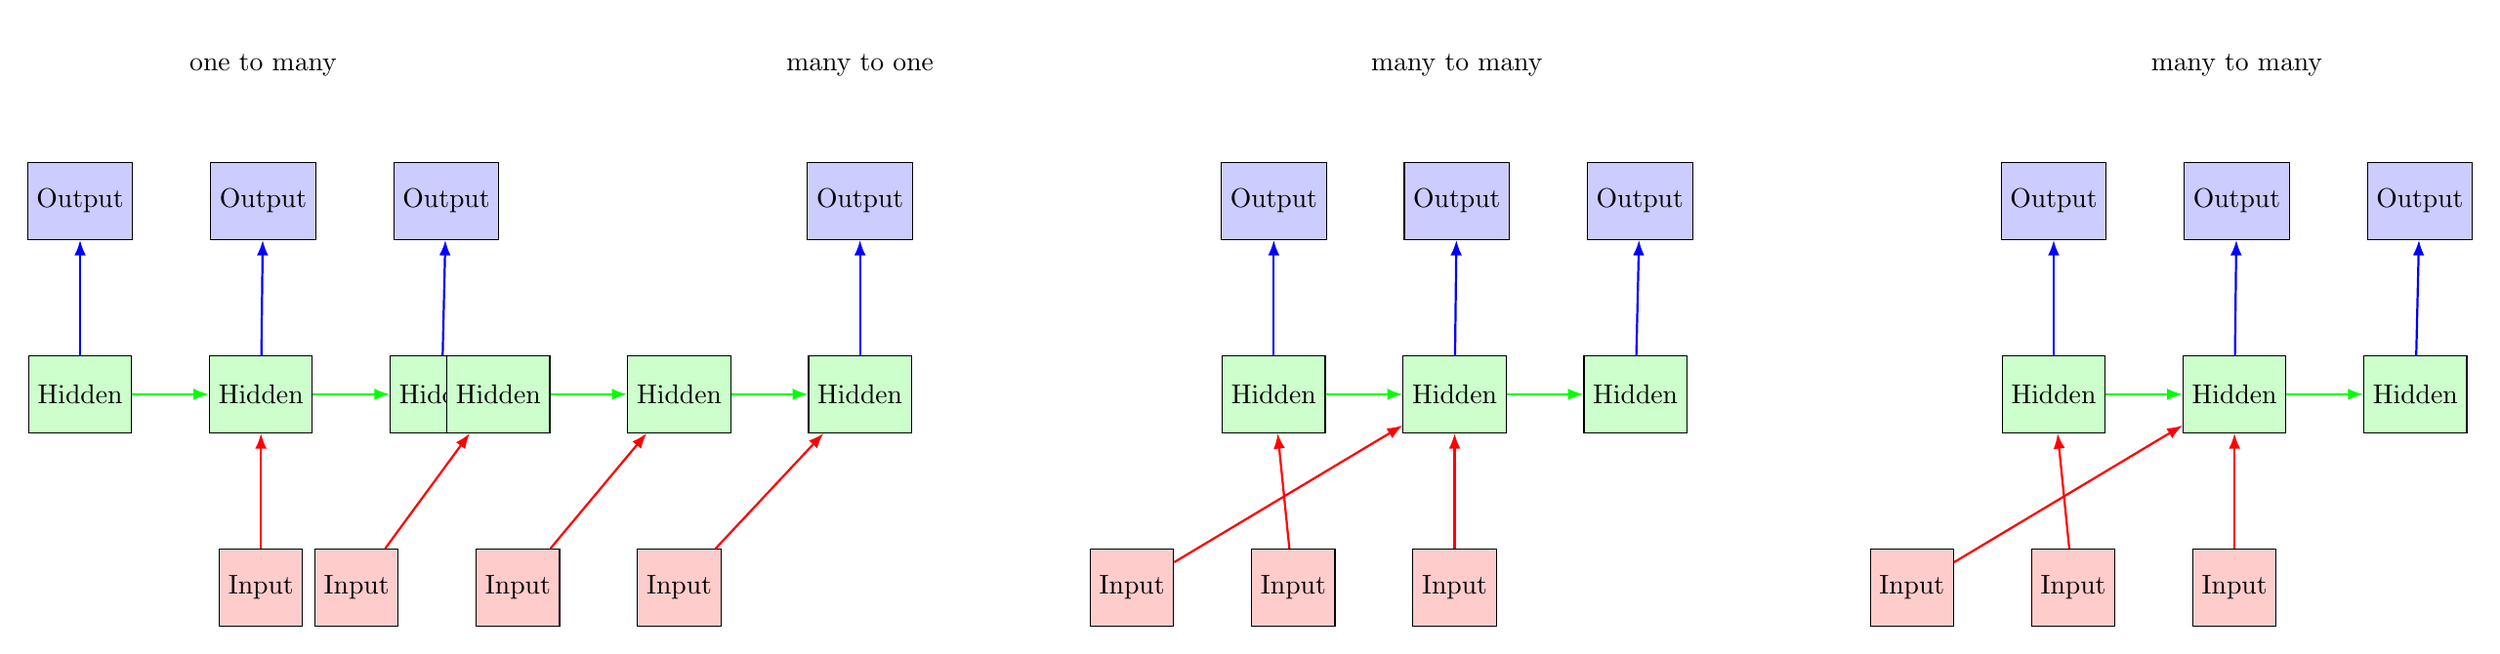
\begin{tikzpicture}[
    node distance=1.5cm and 1cm,
    every node/.style={draw, minimum size=1cm, align=center},
    arrow/.style={-{Latex[length=2mm]}, thick}
]

% One to Many
\node[fill=blue!20] (o21) {Output};
\node[fill=blue!20, right=of o21] (o22) {Output};
\node[fill=blue!20, right=of o22] (o23) {Output};
\node[fill=green!20, below=of o21] (h21) {Hidden};
\node[fill=green!20, right=of h21] (h22) {Hidden};
\node[fill=green!20, right=of h22] (h23) {Hidden};
\node[fill=red!20, below=of h22] (i21) {Input};

\foreach \i/\j in {h21/o21, h22/o22, h23/o23} {
    \draw[arrow, blue] (\i) -- (\j);
}
\foreach \i/\j in {i21/h22} {
    \draw[arrow, red] (\i) -- (\j);
}
\foreach \i/\j in {h21/h22, h22/h23} {
    \draw[arrow, green] (\i) -- (\j);
}
\node[draw=none, above=of o22, yshift=-0.75cm] {one to many};

% Many to One
\node[fill=blue!20, right=4cm of o23] (o11) {Output};
\node[fill=green!20, below=of o11] (h11) {Hidden};
\node[fill=green!20, left=of h11] (h12) {Hidden};
\node[fill=green!20, left=of h12] (h13) {Hidden};
\node[fill=red!20, below=of h12] (i11) {Input};
\node[fill=red!20, left=of i11] (i12) {Input};
\node[fill=red!20, left=of i12] (i13) {Input};

\foreach \i/\j in {h11/o11} {
    \draw[arrow, blue] (\i) -- (\j);
}
\foreach \i/\j in {i11/h11, i12/h12, i13/h13} {
    \draw[arrow, red] (\i) -- (\j);
}
\foreach \i/\j in {h12/h11, h13/h12} {
    \draw[arrow, green] (\i) -- (\j);
}
\node[draw=none, above=of o11, yshift=-0.75cm] {many to one};

% Many to Many
\node[fill=blue!20, right=4cm of o11] (o31) {Output};
\node[fill=blue!20, right=of o31] (o32) {Output};
\node[fill=blue!20, right=of o32] (o33) {Output};
\node[fill=green!20, below=of o31] (h31) {Hidden};
\node[fill=green!20, right=of h31] (h32) {Hidden};
\node[fill=green!20, right=of h32] (h33) {Hidden};
\node[fill=red!20, below=of h32] (i31) {Input};
\node[fill=red!20, left=of i31] (i32) {Input};
\node[fill=red!20, left=of i32] (i33) {Input};

\foreach \i/\j in {h31/o31, h32/o32, h33/o33} {
    \draw[arrow, blue] (\i) -- (\j);
}
\foreach \i/\j in {i31/h32, i32/h31, i33/h32} {
    \draw[arrow, red] (\i) -- (\j);
}
\foreach \i/\j in {h31/h32, h32/h33} {
    \draw[arrow, green] (\i) -- (\j);
}
\node[draw=none, above=of o32, yshift=-0.75cm] {many to many};

% Many to Many (2)
\node[fill=blue!20, right=4cm of o33] (o41) {Output};
\node[fill=blue!20, right=of o41] (o42) {Output};
\node[fill=blue!20, right=of o42] (o43) {Output};
\node[fill=green!20, below=of o41] (h41) {Hidden};
\node[fill=green!20, right=of h41] (h42) {Hidden};
\node[fill=green!20, right=of h42] (h43) {Hidden};
\node[fill=red!20, below=of h42] (i41) {Input};
\node[fill=red!20, left=of i41] (i42) {Input};
\node[fill=red!20, left=of i42] (i43) {Input};

\foreach \i/\j in {h41/o41, h42/o42, h43/o43} {
    \draw[arrow, blue] (\i) -- (\j);
}
\foreach \i/\j in {i41/h42, i42/h41, i43/h42} {
    \draw[arrow, red] (\i) -- (\j);
}
\foreach \i/\j in {h41/h42, h42/h43} {
    \draw[arrow, green] (\i) -- (\j);
}
\node[draw=none, above=of o42, yshift=-0.75cm] {many to many};

\end{tikzpicture}
\end{document}
